\subsubsection{Pengujian pencatatan waktu transaksi}
\label{subsubsection:pengujian-pencatatan-waktu-transaksi}

Pengujian ini mencakup fungsional F-3, yaitu bahwa sistem harus dapat mencatat waktu transaksi dari \textit{request} masuk hingga operasi selesai. Pengujian dibagi dua menjadi pengujian pencatatan waktu transaksi untuk operasi \textit{write} dan operasi \textit{read}. Kode dari pengujian tersebut adalah P-4 dan P-5. Pengujian ini menggunakan \textit{script} pembantu oneshot.js yang sudah dijelaskan pada bagian \ref{subsubsection:implementasi-benchmark}.

Pengujian pencatatan waktu transaksi dengan kode pengujian P-4 dilakukan dengan skenario pengguna mengirimkan \textit{request} \textit{write} ke sistem. Pengujian dilakukan dengan langkah-langkah sebagai berikut:

\begin{enumerate}
  \item Melakukan setup sistem menggunakan \textit{flag} --trace dan --file\_output seperti yang dijelaskan pada bagian \ref{subsection:setup-pengujian}.
  \item Menunggu hingga sistem siap menerima \textit{request}. Konfirmasi dapat dilakukan dengan mengirim \textit{request} HTTP pada \textit{endpoint} /status dan memastikan bahwa sistem sudah memiliki \textit{leader}.
  \item Menjalankan \textit{script} oneshot.js dengan argumen \textit{write} untuk melakukan pengujian operasi dasar. \textit{Script} ini akan mengirimkan \textit{request} \textit{write} ke sistem.
  \item Mengecek \textit{log} yang dihasilkan oleh sistem pada file \textit{output log} dan memastikan bahwa sistem mencatat waktu transaksi.
  \item Mengulangi pengujian dengan sistem \textit{erasure coding} dan juga dengan sistem replikasi.
\end{enumerate}

Hasil yang diharapkan adalah sistem menghasilkan \textit{log} yang memiliki informasi waktu setiap fungsi yang dipanggil dalam sebuah \textit{request} dari masuk hingga selesai. Contoh bentuk \textit{log} yang dihasilkan dapat dilihat pada gambar \ref{fig:log-trace}.

\begin{figure}[ht]
    \centering
    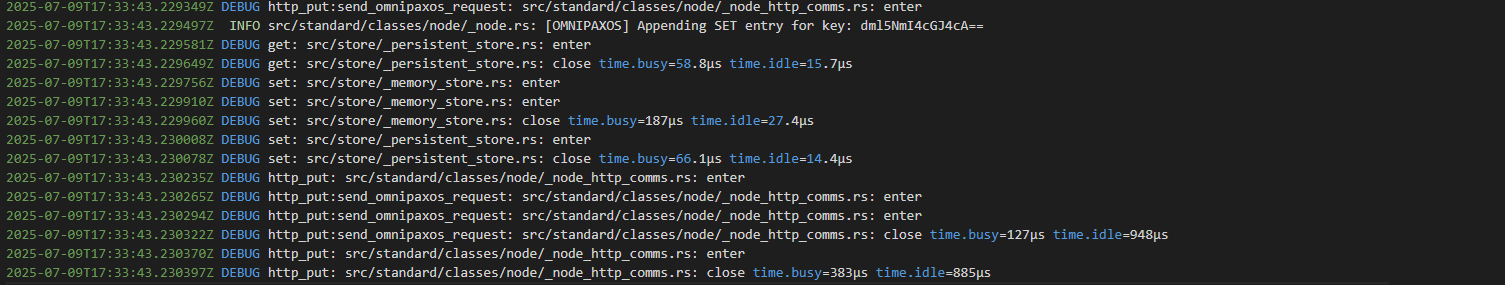
\includegraphics[width=0.95\textwidth]{resources/chapter-4/log-trace.png}
    \caption{Contoh log yang dihasilkan oleh sistem}
    \label{fig:log-trace}
\end{figure}

Pengujian pencatatan waktu transaksi dengan kode pengujian P-5 dilakukan dengan skenario pengguna mengirimkan \textit{request} \textit{read} ke sistem. Pengujian dilakukan dengan langkah-langkah sebagai berikut:

\begin{enumerate}
  \item Melakukan setup sistem menggunakan \textit{flag} --trace dan --file\_output seperti yang dijelaskan pada bagian \ref{subsection:setup-pengujian}.
  \item Menunggu hingga sistem siap menerima \textit{request}. Konfirmasi dapat dilakukan dengan mengirim \textit{request} HTTP pada \textit{endpoint} /status dan memastikan bahwa sistem sudah memiliki \textit{leader}.
  \item Menjalankan \textit{script} oneshot.js dengan argumen \textit{read} untuk melakukan pengujian operasi dasar. \textit{Script} ini akan mengirimkan \textit{request} \textit{read} ke sistem.
  \item Mengecek \textit{log} yang dihasilkan oleh sistem pada file \textit{output log} dan memastikan bahwa sistem mencatat waktu transaksi.
  \item Mengulangi pengujian dengan sistem \textit{erasure coding} dan juga dengan sistem replikasi.
\end{enumerate}

Hasil yang diharapkan adalah sistem menghasilkan \textit{log} yang memiliki informasi waktu setiap fungsi yang dipanggil dalam sebuah \textit{request} dari masuk hingga selesai. Contoh bentuk \textit{log} yang dihasilkan mirip dengan gambar \ref{fig:log-trace} dengan perbedaan pada \textit{request} yang dikirim adalah \textit{read}.